\subsection{Eksperimenta protokols: OpenCV FAST GPU implementācijas ātrdarbība}\label{appx:test2}
\setcounter{table}{0} %Reset table counter for (sub)appendix
\setcounter{figure}{0} %Reset figure counter for (sub)appendix
Eksperimenta mērķis ir novērtēt OpenCV FAST implementāciju GPU platformai.
Šī implementācija ir izstrādāta izpildei ar OpenCL savietojamu 
programmatūras platformu un pavadošo ierīces draiveri. Eksperiments veikts
ar, vienīgo autora rīcībā esošo sistēmu, kurai ir GPU ar OpenCL atbalstu
(sk.~\ref{tbl:test1-dev}~tabulu).
\begin{table}[hb]\small
	\centering
	\caption{Izmantotās iekārtas aprīkojums.}
	\label{tbl:test2-dev}
	\vspace{4pt}
	\begin{tabular}{ll}
		\toprule
		\textbf{CPU} & AMD Phenom II X6 2.80~GHz\\
		\textbf{Video adapteris} & \TODO \\
		\midrule
		\textbf{Operētājsistēma} & Linux 3.8.0 (Ubuntu) \\
		\textbf{Video draiveris} & \TODO \\
		\textbf{OpenCL nodrošinājums} & \TODO \\
		\bottomrule
	\end{tabular}
\end{table}

Par ieejas datiem tika izmantota ,,\termEn{bas-relief}'' attēlu kopa%
	\footnote{Pieejama no \url{http://www.edwardrosten.com/work/junk.tar}}
un uzstādītais jutības slieksnis $t$ visos testos bija 25.
Katram attēla un implementācijas pārim tika veikti 20 mērījumi.
Lielā datu apjoma dēļ (60 ieraksti) visa kopa netiek atspoguļota. Datu
apkopojums redzams \ref{tbl:test2-data}~tabulā, kurā parādīts katra kopas
attēla (20) mērījumu sērijas vidējā vērtība un standartnovirze.

\begin{table}[hb]\footnotesize
	\centering
	\caption{Ātrdarbības rezultāti.}
	\label{tbl:test2-data}
	\vspace{4pt}
	\begin{tabular}{c*{6}{r}}
		\toprule
		\input{results2-t1.tbl_tex}
		\bottomrule
	\end{tabular}
	\begin{minipage}{0.5\linewidth}
		\noindent Apzīmējumi:\\
		$\hat{t_p}$ --- attēla vidējais apstrādes laiks (20 mērījumos)\\
		$\sigma$ --- mērījumu sērijas standartnovirze
	\end{minipage}
\end{table}

Rezultātos var novērot, ka FAST GPU implementācijas ātrdarbība ir līdzīga
CPU implementācijām, bet to nepārsniedz. Tas, iespējams, skaidrojams ar 
datu caurlaidspējas ierobežojumu. Lai gan PCI~Express~x16 (v2.1) datu
maģistrāle atbalsta līdz 64~Gbps datu pārraidi, datu masīva augšupielāde
video kartes (tekstūru) atmiņā var būt krietni lēnāka.
\begin{figure}[t]
	\centering
	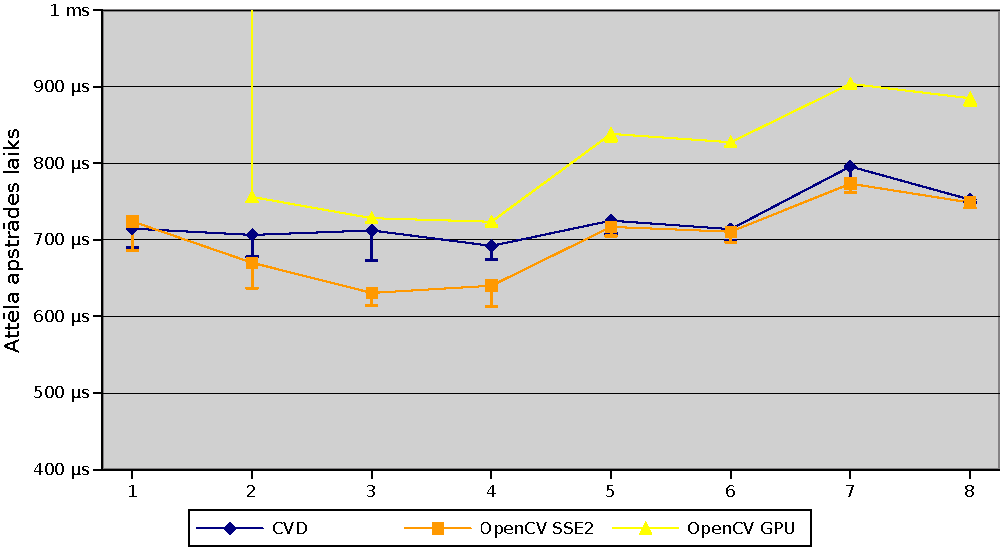
\includegraphics[scale=0.8]{chart-gpu}
	\caption{Attēlu vidējais apstrādes laiks $\hat{t_p}$ dažādiem attēliem.}
	\label{fig:test2-data}
\end{figure}
FAST GPU implementācija arī balstās uz \termEn{integer} tipa aritmētiku, kas
nav tik efektīva, kā peldošā komata skaitļu aritmētika, GPU platformām, bet
šī implementācija, izmanto bitu operācijas, kas \termEn{integer}
aritmētiku padara nepieciešamu.

Mērījumos arī var novērot ļoti augstu apstrādes laiku pirmajam attēlam. Tas
skaidrojams ar to, ka OpenCL kods tiek mērķa ierīcei kompilēts izpildes
laikā. 
Papildus novērojama mazāka standartnovirze GPU implementācijas mērījumiem,
salīdzinot ar CPU implementācijām, jo CPU gadījumā skaitļošanas laiku
izmanto arī operētājsistēma un citas lietojumprogrammas, bet GPU resursi
tiek rezervēti uzdevuma izpildei.

\begin{figure}[bh]
	\centering
	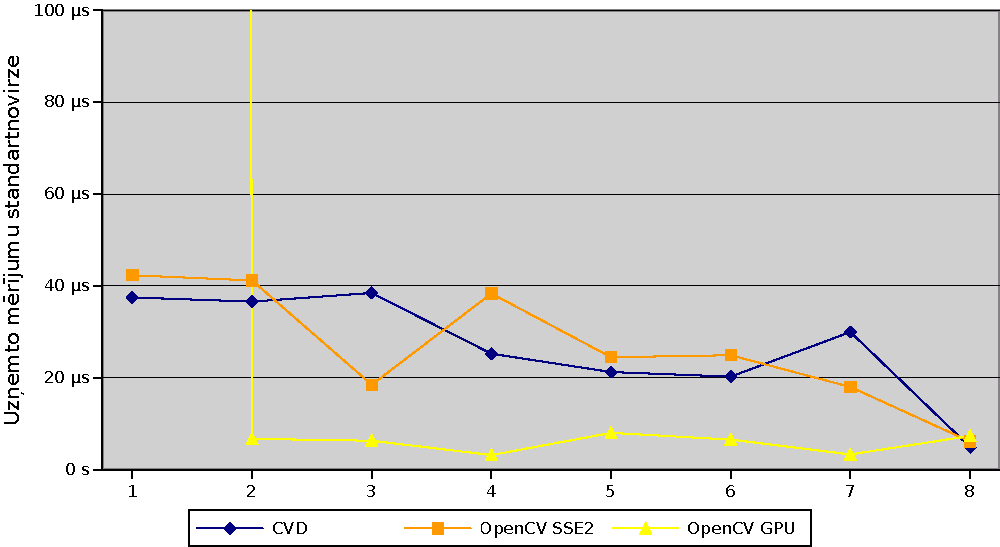
\includegraphics[scale=0.8]{chart-gpu-stdev}
	\caption{Attēlu apstrādes laiku standartnovirze}
	\label{fig:test2-stdev}
\end{figure}
